\begin{frame}{2. 会社の仕事とレオロジー}

\begin{itemize}

\item
  レオロジーとは
\item
  会社の仕事とレオロジー
\item
  レオロジーと商品
\item
  レオロジーとスケール
\end{itemize}

\end{frame}

\begin{frame}{レオロジーとは}

--

\begin{block}{レオロジーの始まり}

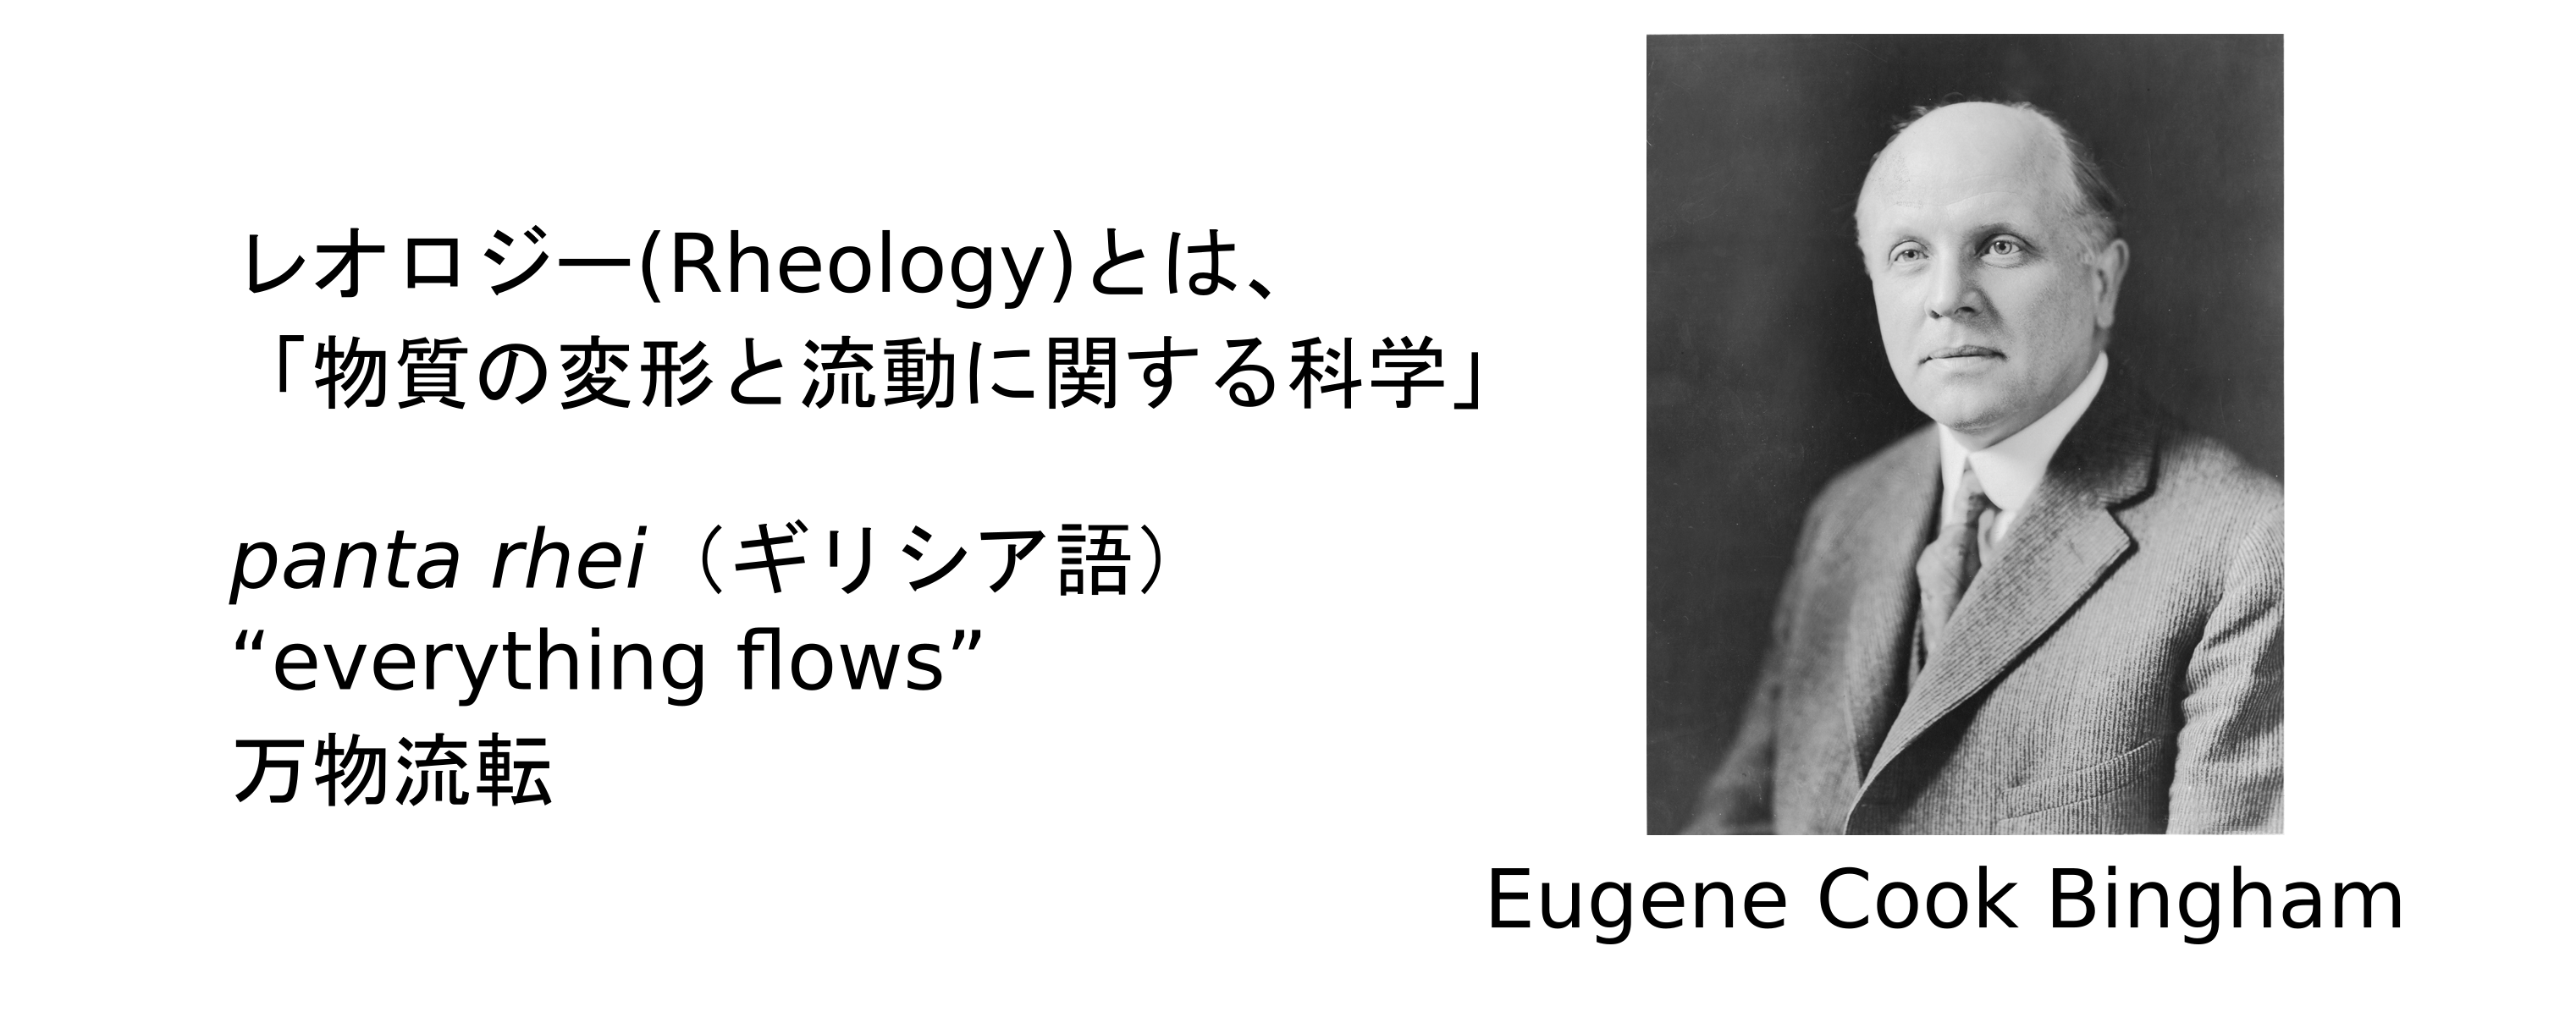
\includegraphics{fig/fig_2/レオロジー.png}

\begin{itemize}

\item
  1929年にアメリカでレオロジー学会が設立
\item
  日本では、1951 年に第1回レオロジー討論会
\end{itemize}

--

\end{block}

\begin{block}{第67回レオロジー討論会}

\begin{itemize}

\item
  協賛:\\
  日本材料学会,プラスチック成形加工学会,高分子学会,日本化学会,日本物理学会,繊維学会,応用物理学会,化学工学会,強化プラスチック協会,日本ゴム協会,日本接着学会,日本セラミックス協会,日本木材学会,セルロース学会,日本機械学会,日本雪氷学会,日本混相流学会,日本流体力学会,可視化情報学会,日本食品科学工学会,日本家政学会,日本調理科学会,日本食品工学会,日本繊維機械学会
\end{itemize}

--

\end{block}

\begin{block}{レオロジーが関連する分野}

\begin{itemize}

\item
  学術分野:化学、物理、生物、化学工学、応用物理、流体力学、地球物理学
\item
  高分子化学(科学):プラスチック、繊維、ゴム、強化プラスチック
\item
  材料:金属、セラミックス、木材
\item
  応用:機械、接着、塗料、食品化学、調理科学、家政学、成型加工
\end{itemize}

--

\end{block}

\begin{block}{非常に幅広い分野が関連}

\begin{itemize}

\item
  レオロジーとは、高度に学際的な科学
\item
  レオロジー技術

  \begin{itemize}
  
  \item
    非常に多様な切り口での議論

    \begin{itemize}
    
    \item
      食品、塗料、心地よさ、潤滑油、等々
    \end{itemize}
  \item
    それぞれの要素技術が異なる⇔内容が多岐
  \item
    一見複雑に見える。
  \end{itemize}
\end{itemize}

\end{block}

\end{frame}

\begin{frame}{会社の仕事とレオロジー}

--

\begin{block}{会社は営利団体で商品を作りたい}

\begin{itemize}

\item
  会社での仕事

  \begin{itemize}
  
  \item
    営利団体(利益を出し続けて、存続)
  \item
    利益を生み出せる商品(製品)を作りたい
  \end{itemize}
\item
  開発のフロー

  \begin{itemize}
  
  \item
    原料⇒材料⇒商品
  \item
    それぞれのステップで評価・解析に基づく、設計を行う。
  \end{itemize}
\item
  そのステップでレオロジーも活用。
\end{itemize}

--

\end{block}

\begin{block}{レオロジーの活用}

--

\end{block}

\begin{block}{「評価・観察」とレオロジー}

例えば、商品に必要な特性をレオロジーで評価

\end{block}

\end{frame}

\begin{frame}{レオロジーと商品}

--

\begin{block}{レオロジーと商品}

\begin{itemize}

\item
  レオロジーを活用して商品を生み出す。

  \begin{itemize}
  \item
    人間の心地よさをレオロジー的感覚で評価
  \item ~
    \subsection{機能設計にレオロジーを利用}
  \end{itemize}
\end{itemize}

\end{block}

\begin{block}{レオロジーと商品(人間の心地よさを定量化)}

\begin{itemize}

\item
  人間の心地よさをレオロジー的感覚で評価

  \begin{itemize}
  
  \item
    「ナタデココ」
  \item
    「トッテモピーチ」(桃の繊維の舌触り)
  \item
    心地よいマッサージ装置
  \item
    肌触りのよい下着
  \item
    伸びの良い下地化粧品
  \end{itemize}
\end{itemize}

--

\end{block}

\begin{block}{レオロジーと商品 (原料、材料の機能設計)}

\begin{itemize}

\item
  機能設計にレオロジーを利用

  \begin{itemize}
  
  \item
    ショックのない運動靴(α-ゲル等)
  \item
    塗り易くて液だれしない塗料
  \item
    ゴワゴワしない着やすい防弾チョッキ
  \item
    よく飛ばせるゴルフクラブ
  \item
    耐震設計、免震設計
  \end{itemize}
\end{itemize}

--

\end{block}

\end{frame}

\begin{frame}{このセクションのまとめ}

\begin{itemize}

\item
  レオロジー技術は非常に多様な切り口での議論

  \begin{itemize}
  
  \item
    食品、塗料、心地よさ、潤滑油、等々
  \item
    それぞれの要素技術が異なる⇔内容が多岐
  \end{itemize}
\item
  実際の商品設計にも多用されている。

  \begin{itemize}
  
  \item
    レオロジーは商品(企業の最終目的)の機能を解析し組み立てるための設計道具である。
  \item
    無くても商品はできるが、あれば便利。
  \end{itemize}
\item
  大きく分けて、

  \begin{itemize}
  
  \item
    人の感覚を定量化
  \item
    原料、材料の機能設計
  \end{itemize}
\end{itemize}

\end{frame}

\begin{frame}{レオロジーとスケール}

--

\begin{block}{マクロとミクロとメゾスケール}

\begin{itemize}

\item
  我々が手で触れるマクロ⇔分子レベルはミクロ
\item
  中間には、メゾスケール
\end{itemize}

--

\end{block}

\begin{block}{材料設計には各種スケールが}

\begin{itemize}

\item
  たいていの場合、最終機能はマクロスケール

  \begin{itemize}
  
  \item
    メゾスケールの多様な構造が機能と関連
  \item
    設計のためには、内部構造の理解も必要
  \end{itemize}
\end{itemize}

--

\end{block}

\end{frame}

\begin{frame}{このセクションのまとめ}

\begin{itemize}

\item
  人間が容易に理解できるのはマクロスケールの事象。

  \begin{itemize}
  
  \item
    人が使う機能の設計もマクロで考えるべき。
  \end{itemize}
\item
  材料の内部では、ミクロからマクロに至るメゾスケールが存在。

  \begin{itemize}
  
  \item
    機能の発現のためにはこのスケールが重要。
  \end{itemize}
\item
  {材料の機能を設計するためにはメゾスケールの理解が必要}

  \begin{itemize}
  
  \item
    「分子レオロジー」
  \end{itemize}
\end{itemize}

\end{frame}
